\documentclass[tikz, border=15pt]{standalone}
\usepackage{tikz}
\usetikzlibrary{calc, shapes.geometric}

\definecolor{wallcolor}{HTML}{E2E8F0}
\definecolor{floorcolor}{HTML}{CBD5E0}
\definecolor{doorframe}{HTML}{718096}
\definecolor{bedcolor}{HTML}{63B3ED}
\definecolor{deskcolor}{HTML}{A0AEC0}
\definecolor{soncloth}{HTML}{ED8936}
\definecolor{vrheadset}{HTML}{1A202C}
\definecolor{momcloth}{HTML}{9F7AEA}
\definecolor{skincolor}{HTML}{FBD38D}

\begin{document}
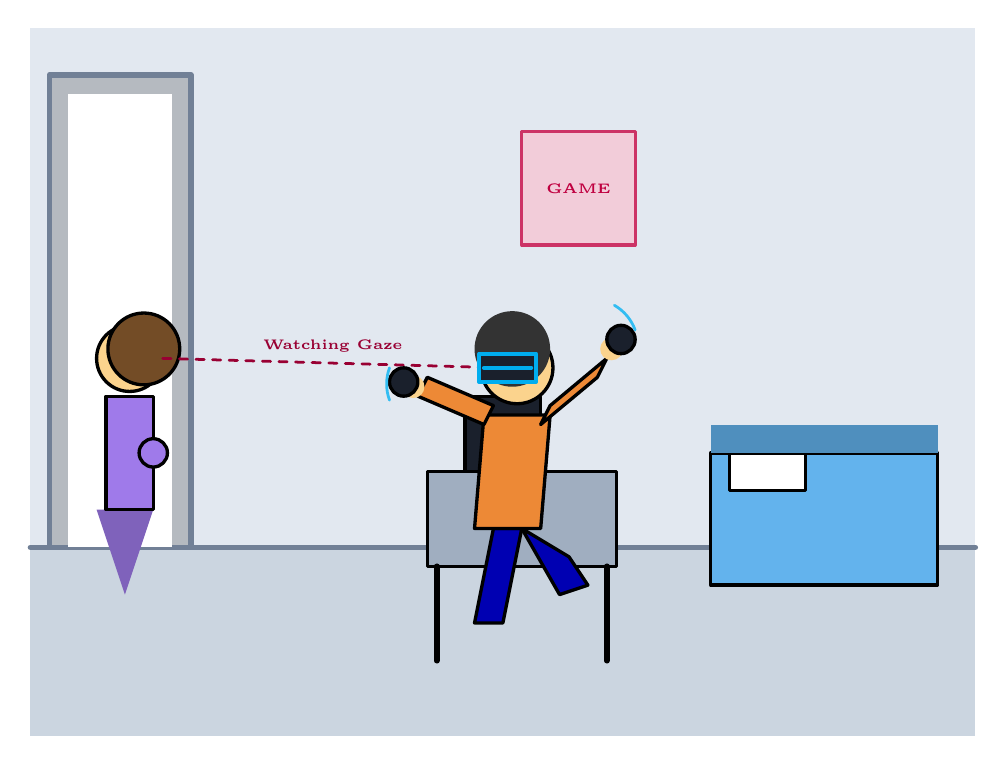
\begin{tikzpicture}[
    scale=1.2,
    line width=1.2pt,
    line join=round,
    line cap=round
]

    % Room Background: Wall and Floor
    \fill[wallcolor] (-5, -2) rectangle (5, 3.5);
    \fill[floorcolor] (-5, -4) rectangle (5, -2);
    \draw[doorframe, line width=2pt] (-5, -2) -- (5, -2);

    % Doorway on Left (Mother standing at entrance)
    \fill[wallcolor!80!black, draw=doorframe, line width=2pt] (-4.8, -2) rectangle (-3.3, 3.0);
    \fill[white] (-4.6, -2) rectangle (-3.5, 2.8); % Open doorway background

    % Kid's Bedroom Furniture (Right & Center)
    % Bed in background right
    \fill[bedcolor, draw=black] (2.2, -2.4) rectangle (4.6, -1.0);
    \fill[white, draw=black] (2.4, -1.4) rectangle (3.2, -1.0); % Pillow
    \fill[bedcolor!80!black] (2.2, -1.0) rectangle (4.6, -0.7); % Blanket fold

    % Desk & Shelf in background center
    \fill[deskcolor, draw=black] (-0.8, -2.2) rectangle (1.2, -1.2);
    \draw[black, line width=2pt] (-0.7, -3.2) -- (-0.7, -2.2);
    \draw[black, line width=2pt] (1.1, -3.2) -- (1.1, -2.2);
    % Monitor on desk
    \fill[vrheadset, draw=black] (-0.4, -1.2) rectangle (0.4, -0.4);
    \draw[black, line width=2pt] (0, -1.2) -- (0, -1.4);

    % Poster on wall
    \fill[purple!20, draw=purple!80] (0.2, 1.2) rectangle (1.4, 2.4);
    \node[purple, font=\tiny\bfseries] at (0.8, 1.8) {GAME};

    % --- MOTHER (Left at Doorway entrance) ---
    % Mother Standing & Peeking in
    \fill[momcloth!80!black] (-4.0, -2.5) -- (-3.7, -1.6) -- (-4.3, -1.6) -- cycle; % Skirt
    \fill[momcloth, draw=black] (-4.2, -1.6) rectangle (-3.7, -0.4); % Torso
    \fill[skincolor, draw=black] (-3.95, 0.0) circle (0.35); % Head
    \fill[brown!60!black, draw=black] (-3.8, 0.1) circle (0.38); % Hair
    % Arms folded / at door edge
    \fill[momcloth, draw=black] (-3.7, -1.0) circle (0.15);
    % Mother's Sightline (Dashed line from Mom to Son)
    \draw[purple!80!black, dashed, line width=1pt] (-3.6, 0.0) -- (0.0, -0.1) node[midway, above, font=\tiny\bfseries] {Watching Gaze};


    % --- SON (Center, Playing with VR) ---
    % Active Pose (One leg bent, body leaning back happily)
    % Legs
    \fill[blue!70!black, draw=black] (-0.3, -2.8) -- (-0.1, -1.8) -- (0.2, -1.8) -- (0.0, -2.8) -- cycle;
    \fill[blue!70!black, draw=black] (0.2, -1.8) -- (0.7, -2.1) -- (0.9, -2.4) -- (0.6, -2.5) -- cycle;

    % Torso (Shirt)
    \fill[soncloth, draw=black] (-0.3, -1.8) -- (0.4, -1.8) -- (0.5, -0.6) -- (-0.2, -0.6) -- cycle;

    % Head with VR Headset
    \fill[skincolor, draw=black] (0.15, -0.1) circle (0.38);
    \fill[black!80] (0.1, 0.1) circle (0.40); % Hair
    % VR Headset strap & visor
    \fill[vrheadset, draw=cyan, line width=1.5pt] (-0.25, -0.25) rectangle (0.35, 0.05);
    \draw[cyan, line width=1.5pt] (-0.2, -0.1) -- (0.3, -0.1); % LED glow strip on VR headset

    % Left Arm extended forward with Controller
    \fill[soncloth, draw=black] (-0.2, -0.7) -- (-0.9, -0.4) -- (-0.8, -0.2) -- (-0.1, -0.5) -- cycle;
    \fill[skincolor] (-0.95, -0.3) circle (0.12);
    \fill[vrheadset, draw=black] (-1.05, -0.25) circle (0.15); % Controller

    % Right Arm raised up with Controller
    \fill[soncloth, draw=black] (0.4, -0.7) -- (1.0, -0.2) -- (1.1, 0.0) -- (0.5, -0.5) -- cycle;
    \fill[skincolor] (1.15, 0.1) circle (0.12);
    \fill[vrheadset, draw=black] (1.25, 0.2) circle (0.15); % Controller

    % Motion Effect Lines around Son
    \draw[cyan!80, line width=1pt] (-1.2, -0.1) arc (160:200:0.5);
    \draw[cyan!80, line width=1pt] (1.4, 0.3) arc (20:60:0.5);

\end{tikzpicture}
\end{document}
